\documentclass[10pt]{beamer}
\usetheme{jambro}

\title[]{Macroeconomia I - Curva de Phillips, taxa natural de desemprego e inflação}
\author[]{\href{https://pvfonseca.github.io}{Paulo Victor da Fonseca}}
\date{}

\hypersetup{
    colorlinks = true,
    urlcolor = teal,
    linkcolor = teal    
}
\usepackage[portuguese]{babel}
\usepackage{subfig}
\usepackage{emoji}
\usepackage{hyperref}

\begin{document}

\begin{frame}[plain]
    \titlepage{
        \begin{center}
            \begin{minipage}{0.8\textwidth}
                \centering
            \end{minipage}
        \end{center}}
\end{frame}

\begin{frame}{Sumário}
    \tableofcontents
\end{frame}

\section{A curva de Phillips e a taxa natural de desemprego}
\subsection{A curva de Phillips e a taxa natural de desemprego}
\begin{frame}{Curva de Phillips e taxa natural de desemprego}
    \begin{itemize}
        \item A curva de Phillips (PC) está intimamente ligada com a taxa natural de desemprego.
        \bigskip
        \item A PC original implicava que não existia algo como uma taxa natural de desemprego para o qual a economia convergiria no médio prazo.
        \bigskip
        \item Se os formuladores de política econômica estivessem dispostos a tolerar uma taxa de inflação mais alta, poderiam manter uma taxa de desemprego mais baixa para sempre.
        \bigskip
        \item Este trade-off parecia ser corroborado pela evidência empírica da década de 1960.
    \end{itemize}
\end{frame}

\begin{frame}{Curva de Phillips e taxa natural de desemprego}
    \begin{itemize}
        \item No entanto, em 1968, dois economistas questionaram a existência de um trade-off estável entre desemprego e inflação.
    \end{itemize}
    \begin{figure}
        \centering
        \subfloat[Milton Friedman (1912-2006)\label{fig1a}]{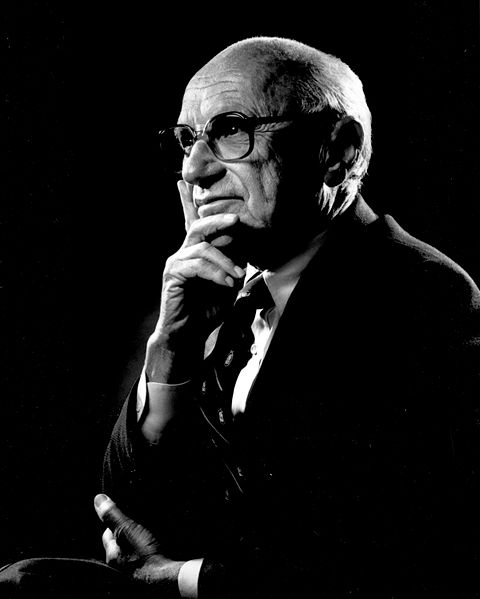
\includegraphics[width=0.24\textwidth]{./figures/macro14_fig1.jpg}}\qquad
        \subfloat[Edmund Phelps (1933 - )\label{fig3b}]{
\includegraphics[width=0.3\textwidth]{./figures/macro14_fig2.jpg}}
        \caption{Milton Friedman e Edmund Phelps - Prêmio Nobel de Economia em 1976 e 2006, respectivamente.}
        \label{fig1b}
    \end{figure}
\end{frame}

\begin{frame}{Curva de Phillips e taxa natural de desemprego}
    \begin{itemize}
        \item As conclusões de Friedman e Phelps são uns dos raros exemplos em economia de teorias desenvolvidas \emph{ex-ante}. Normalmente, a maioria de nossas percepções são derivadas após o acontecimento dos fatos.
        \bigskip
        \item Friedman e Phelps questionaram a existência de um trade-off permanente entre inflação e desemprego argumentando que este trade-off só poderia existir se os fixadores de salários subestimassem sistematicamente a inflação, sendo pouco provável que cometessem o mesmo erro para sempre.
        \bigskip
        \item Além disso, se o governo tentasse sustentar o desemprego mais baixo aceitando uma inflação mais alta, o trade-off acabaria por desaparecer.
        \bigskip
        \item A taxa de desemprego não poderia ser sustentada abaixo de determinado nível, um nível que eles chamaram \textcolor{blue}{taxa natural de desemprego}.
    \end{itemize}
\end{frame}

\begin{frame}{Curva de Phillips e taxa natural de desemprego}
    \begin{itemize}
        \item Como vimos anteriormente, a taxa natural de desemprego, $u_n$, é a taxa de desemprego em que o nível de preços efetivo é igual ao nível esperado de preços: $P = P^e$.
        \bigskip
        \item De modo análogo, $u_n$ é a taxa de desemprego associada à situação em que $\pi = \pi^e$.
        \bigskip
        \item Na aula passada vimos que:
        \begin{equation}
        \pi_t = \pi^e_t + (m + z) - \alpha u_t.
        \label{eq1}
        \end{equation}
        \bigskip
        \item Portanto, a taxa natural de desemprego é tal que:
        \begin{equation*}
            0 = (m + z) - \alpha u_n.
        \end{equation*}
        \bigskip
        \item Ou seja, a taxa natural de desemprego é uma constante definida por:
        \begin{equation}
            u_n = \frac{m + z}{\alpha}.
            \label{eq2}
        \end{equation}
    \end{itemize}
\end{frame}

\begin{frame}{Curva de Phillips e taxa natural de desemprego}
    \begin{itemize}
        \item Pela equação (\ref{eq2}), quanto maior o markup, $m$, ou os fatores que afetam a fixação de salários, $z$, maior será a taxa natural de desemprego.
        \bigskip
        \item Quanto maior a força do efeito do desemprego sobre o salário, $\alpha$, menor será a taxa de desemprego natural.
        \bigskip
        \item Podemos reescrever a equação (\ref{eq1}) da seguinte maneira:
        \[
        \pi_t - \pi^e_t = -\alpha \left(u_t - \frac{m + z}{\alpha}\right).
        \]
        \bigskip
        \item Portanto:
        \begin{equation}
            \pi_t - \pi^e_t = -\alpha (u_t - u_n).
            \label{eq3}
        \end{equation}
    \end{itemize}
\end{frame}

\begin{frame}{Curva de Phillips e taxa natural de desemprego}
    \begin{itemize}
        \item Se a taxa de inflação esperada, $\pi^e_t$, puder ser aproximada pela taxa de inflação do período anterior, $\pi_{t-1}$, obtemos:
        \begin{eqnarray}
            \Delta \pi_t \equiv \pi_t - \pi_{t-1} = -\alpha (u_t - u_n), \label{eq4}
        \end{eqnarray}
        \bigskip
        \item A variação na taxa de inflação depende do desvio entre a taxa de desemprego efetiva e a taxa de desemprego natural.
        \bigskip
        \item Quando a taxa de desemprego efetiva é maior que a taxa natural, a taxa de inflação diminui.
        \bigskip
        \item Por outro lado, se a taxa de desemprego efetiva é menor que a taxa natural, a taxa de inflação aumenta.
        \bigskip
        \item Por fim, podemos interpretar a taxa natural de desemprego como a taxa de desemprego necessária para manter a taxa de inflação constante - \textcolor{blue}{taxa de desemprego não aceleradora da inflação (NAIRU)}.
    \end{itemize}
\end{frame}

\begin{frame}{Curva de Phillips e taxa natural de desemprego}
    \begin{itemize}
        \item Na aula passada vimos que a reta de regressão que melhor se ajusta aos dados de taxa de desemprego e variação na taxa de inflação para a economia norte-americana para o período 1970-2014 é dada por:
        \[
        \Delta \pi_t = 3,0\% - 0,5u_t.
        \]
        \bigskip
        \item Isso implica que, nos EUA de 1970-2014, a taxa média de desemprego necessária para manter a inflação constante é igual a 6\%.
    \end{itemize}
\end{frame}

\begin{frame}{Curva de Phillips e taxa natural de desemprego}
    \begin{itemize}
        \item Como vimos, a taxa natural de desemprego depende de todos os fatores que afetam a fixação de salários, representados pela variável $z$; do markup, $m$, e da resposta da inflação ao desemprego, $\alpha$.
        \bigskip
        \item Portanto, não há motivos para esperarmos que todos os países tenham a mesma taxa natural de desemprego.
        \bigskip
        \item As taxas naturais diferem entre países, às vezes de modo considerável.
    \end{itemize}
\end{frame}

\begin{frame}{Curva de Phillips e taxa natural de desemprego}
    \begin{figure}
        \centering
        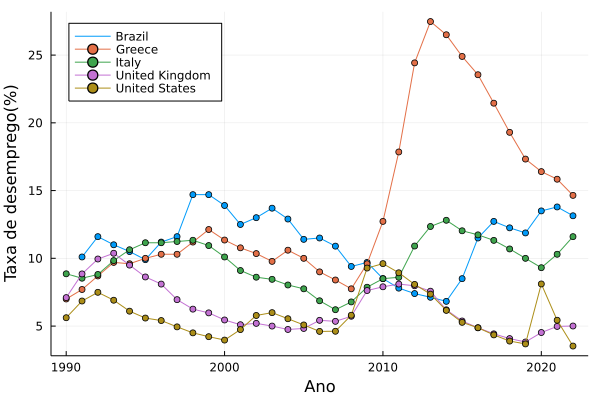
\includegraphics[width=0.65\textwidth]{./figures/macro14_fig3.png}
        \caption{Dinâmica das taxas de desemprego, 1990-2022. Fonte: \href{https://www.imf.org/en/Publications/SPROLLS/world-economic-outlook-databases\#sort=\%40imfdate\%20descending}{FMI - World Economic Outlook} (Elaboração própria).}
        \label{fig2}
    \end{figure}
\end{frame}

\begin{frame}{Curva de Phillips e taxa natural de desemprego}
    \begin{itemize}
        \item Uma taxa de desemprego alta por alguns anos pode indicar um desvio com relação à taxa natural.
        \bigskip
        \item Já uma taxa de desemprego alta por um longo período de tempo, associada a nenhuma diminuição sustentada da inflação, reflete uma alta taxa natural.
        \bigskip
        \item Neste caso, devemos procurar explicações para uma taxa natural elevada nas relações de fixação de salários e fixação de preços.
        \bigskip
        \item Para o caso europeu, é comum ouvirmos falar que um dos principais problemas é a rigidez do mercado de trabalho.
        \bigskip
        \item Embora essa afirmativa seja parcialmente verdadeira, a realidade é mais complexa.
    \end{itemize}
\end{frame}

\begin{frame}{Curva de Phillips e taxa natural de desemprego}
    \begin{itemize}
        \item Por rigidez no mercado de trabalho os economistas se referem aos seguintes itens:
        \bigskip
        \begin{enumerate}
            \item Um generoso sistema de seguro-desemprego: a taxa de reposição (relação entre o seguro-desemprego e o salário após impostos) costuma ser alta na Europa, e a duração dos benefícios frequentemente dura anos.
            \bigskip
            \item Um alto grau de proteção ao emprego: as evidências sugerem que embora a proteção ao emprego não necessariamente aumente o desemprego, ela altera sua natureza - a oscilação do desemprego diminui, mas sua duração média aumenta (o que aumenta a probabilidade de os desempregados perderem suas habilidades e autoestima, afetando sua empregabilidade).
            \bigskip
            \item Salário mínimo. Em alguns países, a relação entre o salário mínimo e a renda mediana pode ser bastante alta.
            \bigskip
            \item Regras de negociação. Na maior parte dos países europeus, os contratos de trabalho estão sujeitos a acordos de extensão, o que aumenta o poder de negociação dos sindicatos, pois reduz o escopo para competição por parte das empresas não sindicalizadas.
        \end{enumerate}
    \end{itemize}
\end{frame}

\begin{frame}{Curva de Phillips e taxa natural de desemprego}
    \begin{itemize}
        \item Essas instituições do mercado de trabalho realmente explicam o alto desemprego na Europa?
        \bigskip
        \begin{enumerate}
            \item O desemprego nem sempre foi alto na Europa. Na década de 60 era cerca de 2\% a 3\% nos quatro principais países continentais. Hoje está em torno de 8\% a 9\%.
            \bigskip
            \item Antes do início da CFG, uma série de países europeus apresentava baixo desemprego - ver figura a seguir com dados de 2006 (inflação estável, sugerindo que a taxa de desemprego era próxima da taxa natural).
        \end{enumerate}
    \end{itemize}
\end{frame}

\begin{frame}{Curva de Phillips e taxa natural de desemprego}
    \begin{figure}
        \centering
        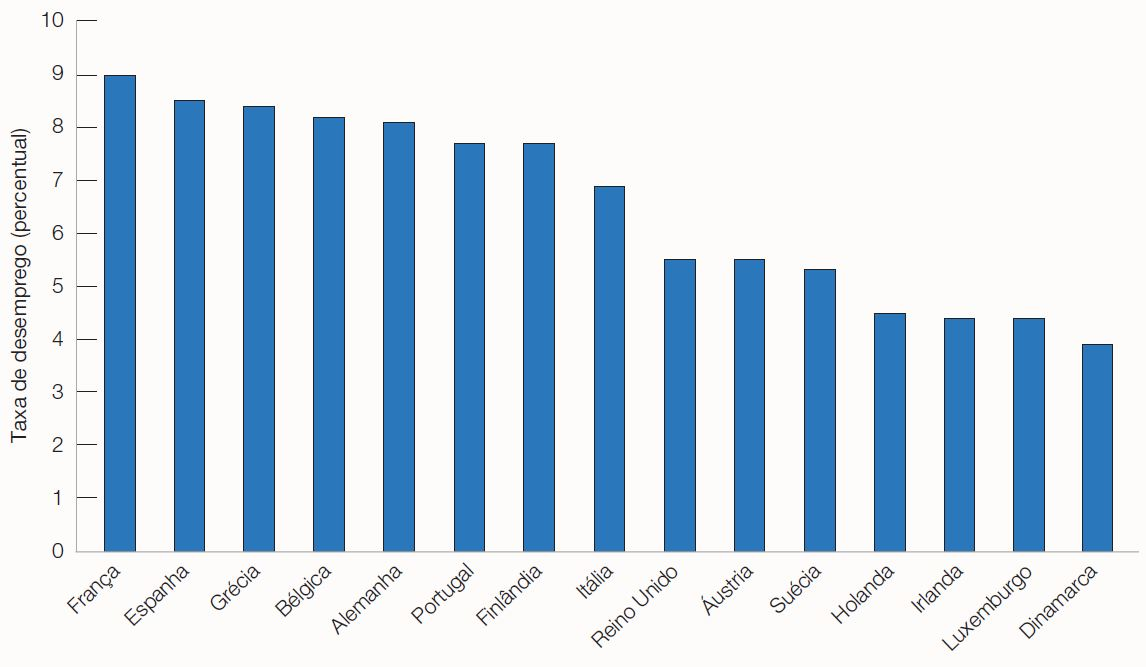
\includegraphics[width=0.8\textwidth]{./figures/macro14_fig4.JPG}
        \caption{Taxa de desemprego em 15 países europeus, 2006. Fonte: Blanchard (2017).}
        \label{fig3}
    \end{figure}
\end{frame}

\subsection{Dinâmica da taxa natural de desemprego}
\begin{frame}{Dinâmica da taxa natural de desemprego}
    \begin{itemize}
        \item A estimativa da curva de Phillips modificada que vimos anteriormente assume, implicitamente, que $m + z$ é uma constante.
        \bigskip
        \item No entanto, existem bons motivos para crer que $m$ e $z$ variem ao longo do tempo.
        \bigskip
        \item O grau do poder de monopólio das empresas, os custos de insumos que não a mão de obra, a estrutura das negociações salariais, o sistema de seguro-desemprego, etc. provavelmente variam ao longo do tempo, o que implica que $m$ ou $z$ e, consequentemente, a taxa natural de desemprego também varie ao longo do tempo.
        \bigskip
        \item As variações da taxa natural de desemprego ao longo do tempo são difíceis de mensurar pois esta é uma variável não observável. Só observamos a taxa de desemprego efetiva.
        \bigskip
        \item Mas mudanças em linhas gerais podem ser determinadas comparando-se as taxas médias de desemprego de uma década para a outra.
    \end{itemize}
\end{frame}

\subsection{Inflação alta e curva de Phillips}
\begin{frame}{Inflação alta e curva de Phillips}
    \begin{itemize}
        \item Vimos que na década de 1970, a curva de Phillips dos EUA mudou à medida que a inflação se tornou mais persistente, e os fixadores de salários mudaram a maneira como formavam suas expectativas acerca da inflação.
        \bigskip
        \item Essa é uma lição genérica, a relação entre desemprego e inflação provavelmente muda com o nível e a persistência da inflação.
        \bigskip
        \item A evidência de países com inflação alta confirma essa lição.
        \bigskip
        \item Não somente muda a maneira como trabalhadores e empresas formam suas expectativas mas, também, mudam-se os arranjos institucionais.
    \end{itemize}
\end{frame}

\begin{frame}{Inflação alta e curva de Phillips}
    \begin{itemize}
        \item Quando a inflação se eleva, a inflação tende a ser mais volátil.
        \bigskip
        \item Portanto, os trabalhadores e empresas ficam mais relutantes em fechar contratos de trabalho que fixem salários nominais por um longo período de tempo.
        \bigskip
        \item Por isso, nos EUA, os termos dos acordos salariais mudam com o nível de inflação.
        \bigskip
        \item Os salários nominais são fixados por períodos de tempo mais curtos, indo de um ano a um mês, ou até menos.
        \bigskip
        \item A \textbf{indexação de salários}, uma cláusula que aumenta automaticamente os salários de acordo com a inflação, torna-se mais difundida.
        \bigskip
        \item Essas mudanças levam, por sua vez, a uma resposta mais forte da inflação ao desemprego.
    \end{itemize}
\end{frame}

\begin{frame}{Inflação alta e curva de Phillips}
    \begin{itemize}
        \item Suponha que uma proporção $\lambda$ dos contratos de trabalho é indexada à inflação, ou seja, os salários nominais ajustam-se proporcionalmente à variação do nível de preços efetivo.
        \bigskip
        \item A fração restante, $1 - \lambda$, dos contratos de trabalho é não indexada, ou seja, os salários nominais são fixados com base na inflação esperada.
        \bigskip
        \item Formalmente, temos:
        \begin{equation}
            \pi_t = [\lambda\pi_t + (1-\lambda)\pi_t^e] - \alpha(u_t - u_n).
            \label{eq5}
        \end{equation}
        \bigskip
        \item Assumindo expectativas adaptativas, $\pi_t^e = \pi_{t-1}$, temos:
        \begin{equation}
            \pi_t = [\lambda\pi_t + (1-\lambda)\pi_{t-1}] - \alpha(u_t - u_n).
            \label{eq6}
        \end{equation}
    \end{itemize}
\end{frame}

\begin{frame}{Inflação alta e curva de Phillips}
    \begin{itemize}
        \item Se todos os salários são não indexados, temos:
        \[
        \pi_t - \pi_{t-1} = -\alpha (u_t - u_n).
        \]
        \bigskip
        \item No entanto, quando uma fração positiva dos salários são indexados, temos que:
        \[
        \pi_t - \pi_{t-1} = -\frac{\alpha}{1-\lambda}(u_t-u_n).
        \]
        \bigskip
        \item \textcolor{blue}{A indexação de salários aumenta o efeito do desemprego sobre a inflação}.
    \end{itemize}
\end{frame}

\begin{frame}{Inflação alta e curva de Phillips}
    \begin{itemize}
        \item Sem indexação de salários, o desemprego menor aumenta os salários o que, por sua vez, aumenta os preços.
        \bigskip
        \item No entanto, como os salários não respondem imediatamente aos preços, não há um aumento adicional de preços dentro do ano.
        \bigskip
        \item Com a indexação de salários, entretanto, um aumento de preços leva a um aumento adicional dos salários dentro do ano, o que leva a um aumento adicional nos preços, e assim por diante, de modo que o efeito do desemprego sobre a inflação dentro do ano é maior.
        \bigskip
        \item Se $\lambda \to 1$, pequenas mudanças no desemprego podem levar a variações muito grandes da inflação. Dito de outra maneira, pode haver grandes variações da inflação com praticamente nenhuma mudança no desemprego.
        \bigskip
        \item Isto é o que acontece em países onde a inflação é muito alta.
        \bigskip
        \item A inflação entre desemprego e inflação torna-se muito tênue até, finalmente, desaparecer por completo.
    \end{itemize}
\end{frame}

\subsection{Deflação e curva de Phillips}
\begin{frame}{Deflação e curva de Phillips}
    \begin{itemize}
        \item O que acontece com a curva de Phillips quando a inflação é muito baixa ou, até mesmo, há deflação?
        \bigskip
        \item A motivação pra essa questão é dada por eventos como os da Grande Depressão.
        \bigskip
        \item Na Figura \ref{fig4} vemos um desemprego excessivamente alto e, dada essa taxa de desemprego, a taxa de inflação está surpreendentemente alta.
        \bigskip
        \item Dito de outra forma, dado um desemprego muito alto, teríamos esperado não somente uma deflação mas, também, uma alta da taxa de deflação.
        \bigskip
        \item Na verdade, a deflação foi limitada, e de 1934 a 1937, apesar de um desemprego ainda elevado, a inflação foi positiva.
    \end{itemize}
\end{frame}

\begin{frame}{Deflação e curva de Phillips}
    \begin{figure}
        \centering
        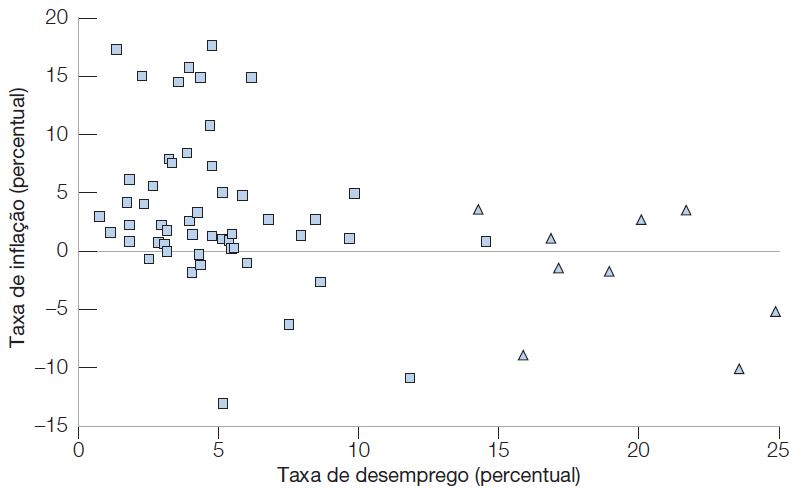
\includegraphics[width=0.7\textwidth]{./figures/macro14_fig5.JPG}
        \caption{Inflação $\times$ desemprego, EUA (1900-1960). Fonte: Blanchard (2017).}
        \label{fig4}
    \end{figure}
\end{frame}

\begin{frame}{Deflação e curva de Phillips}
    \begin{itemize}
        \item Existem duas explicações possíveis para estes eventos:
        \bigskip
        \begin{enumerate}
            \item A Grande Depressão estava associada a um aumento não só da taxa de desemprego mas, também, da taxa natural de desemprego. Isso parece improvável, a maioria dos economistas vê os anos 1930 como resultado de um grande deslocamento adverso da demanda agregada que levou a um aumento da taxa de desemprego efetiva em relação à taxa natural.
            \bigskip
            \item \textbf{Quando a economia começa a experimentar deflação, a relação da curva de Phillips quebra}. Uma possível razão é a relutância dos trabalhadores em aceitar redução dos salários nominais. Eles aceitam inconscientemente um corte nos salários reais, entretanto, lutarão contra o mesmo corte nos salários reais se estes resultarem de um corte explícito em seus salários nominais. Esse mecanismo é claramente ativo em alguns países.
        \end{enumerate}
    \end{itemize}
\end{frame}

\begin{frame}{Deflação e curva de Phillips}
    \begin{figure}
        \centering
        \subfloat[Alta inflação (27\%) - Portugal (1984)\label{fig5a}]{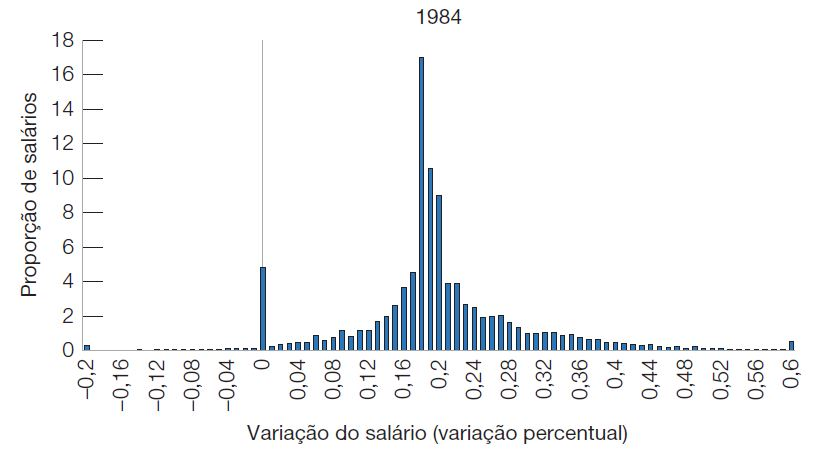
\includegraphics[width=0.45\textwidth]{./figures/macro14_fig6.JPG}}\qquad
        \subfloat[Baixa inflação (2,1\%) - Portugal (2012)\label{fig5b}]{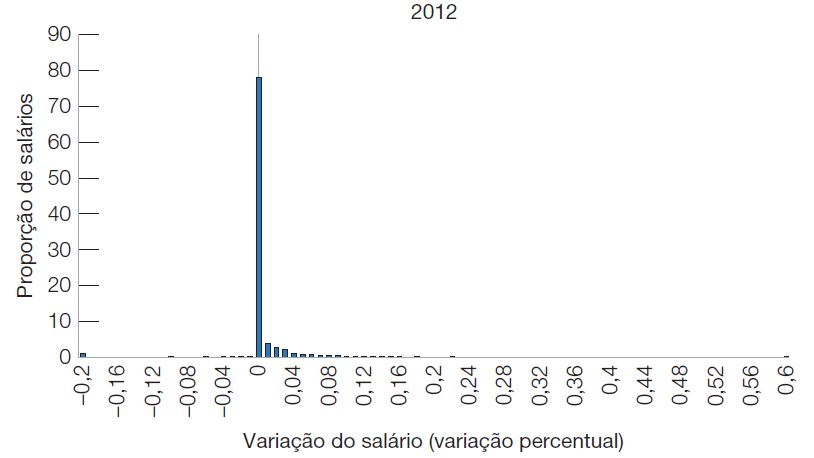
\includegraphics[width=0.45\textwidth]{./figures/macro14_fig7.JPG}}
        \caption{Distribuição das variações salariais em Portugal. Fonte: Blanchard (2017).}
        \label{fig5}
    \end{figure}
\end{frame}

\begin{frame}{Deflação e curva de Phillips}
    \begin{itemize}
        \item A Figura \ref{fig5} mostra a distribuição das variações salariais em Portugal em tempos de baixa e alta inflação.
        \bigskip
        \item Em 1984, quando a inflação era de 27\%, a distribuição das variações salariais é aproximadamente simétrica - Figura \ref{fig5a}.
        \bigskip
        \item Já para 2012, quando a inflação era de apenas 2,1\%, a distribuição das variações salariais é agrupada em zero, com quase nenhuma variação salarial negativa.
        \bigskip
        \item Na medida em que esse mecanismo está ativo, isso implica que a relação da curva de Phillips entre a variação da inflação e o desemprego pode desaparecer ou, pelo menos, tornar-se mais fraca, quando a economia está próxima da inflação zero.
        \bigskip
        \item Quando a inflação é baixa, poucos trabalhadores aceitam um corte nos salários nominais.
    \end{itemize}
\end{frame}

\begin{frame}{Deflação e curva de Phillips}
    \begin{itemize}
        \item Essa questão não é apenas de interesse histórico.
        \bigskip
        \item Durante a CFG, o desemprego aumentou consideravelmente em alguns países.
        \bigskip
        \item Esperava-se que isso provocasse uma grande redução da inflação, na verdade, uma deflação substancial.
        \bigskip
        \item No entanto, mesmo que alguns países tenham passado por deflação, ela foi limitada.
        \bigskip
        \item De modo geral, a inflação foi mais elevada do que teria sido prevista pelas curvas de Phillips estimadas para cada país.
        \bigskip
        \item Se isso se deve ao mecanismo que acabamos de descrever, ou se reflete uma mudança na formação de expectativas dos agentes (uma diminuição do $\theta$) continua uma incógnita.
    \end{itemize}
\end{frame}

\section{Bibliografia}
\begin{frame}{\emoji{books} Bibliografia}
    \begin{itemize}                
        \item BLANCHARD, O. Macroeconomia. 7.ed. São Paulo: Pearson Education do Brasil, 2017\medskip                
        \item CARLIN, W.; SOSKICE, D. Macroeconomics: Institutions, instability, and the financial system. Oxford, UK: Oxford University Press, 2015\medskip        
        \item DORNBUSCH, R.; FISCHER, S.; STARTZ, R. Macroeconomia. 11.ed. Porto Alegre: AMGH, 2013. Disponível em: \href{https://app.minhabiblioteca.com.br/books/9788580551853}{app.minhabiblioteca.com.br/books/9788580551853}\medskip
        \item FROYEN, R. Macroeconomia: teorias e aplicações. 2.ed. São Paulo: Saraiva, 2013. Disponível em: \href{https://app.minhabiblioteca.com.br/books/9788502175235}{app.minhabiblioteca.com.br/books/9788502175235}        
    \end{itemize}
\end{frame}
\end{document}